\documentclass[11pt,a4paper]{article}

\usepackage[utf8]{inputenc}
\usepackage[english]{babel}
\usepackage[margin=2.5cm]{geometry}
\usepackage{tabularx}
\usepackage{hyperref}
\usepackage{url}
\usepackage{graphicx}
\usepackage{listings}
\usepackage{xcolor}
\usepackage{indentfirst}
\usepackage{amsmath}

\nocite{*}
\hypersetup{pdfborder=0 0 0}

\lstset{
    backgroundcolor=\color{lightgray!20},
    basicstyle=\ttfamily\small,
    keywordstyle=\color{blue}\bfseries,
    commentstyle=\color{green!50!black},
    stringstyle=\color{red},
    numbers=none,
    numberstyle=\tiny\color{gray},
    frame=single,
    breaklines=true
}

\lstdefinelanguage{Python}{
    keywords={import, from, as, def, return, if, else, elif, for, while, in, try, except, with, class},
    keywordstyle=\color{blue}\bfseries,
    comment=[l]{\#},
    commentstyle=\color{green!50!black},
    stringstyle=\color{red},
    morestring=[b]',
    morestring=[b]"
}

\lstdefinelanguage{Bash}{
    % Remove the keywords list entirely
    comment=[l]{\#},
    commentstyle=\color{green!50!black},
    stringstyle=\color{red},
    morestring=[b]',
    morestring=[b]",
    % Define @ as an invisible delimiter for your keyword style
    moredelim=[is][\color{blue}\bfseries]{@}{@}
}

% Title Page Information
\title{
    \vspace{-2cm}
    \textbf{Instituto Superior de Engenharia do Porto} \\
    Politécnico do Porto \\
    \vspace{0.5cm}
    Licenciatura em Engenharia Electrotécnica e de Computadores \\
    Sistemas Computacionais Avançados (SISTCA) / Advanced Computing Systems \\
    \vspace{1cm}
    \Large{\textbf{Lab Classes Script: Hand Tracking Using Computer Vision}} \\
}
\author{}
\date{}

\begin{document}

\maketitle

% Version Control Section
\section*{Version Control}
\begin{center}
\renewcommand{\arraystretch}{1.5}
\begin{tabularx}{\textwidth}{|l|l|X|X|}
\hline
\textbf{Version number} & \textbf{Date issued} & \textbf{Authors} & \textbf{Update information} \\ \hline
V1.0 & April 2026 & Rodrigo Pires (1210697) \newline Miguel Veloso (1212013) \newline Rui Rodrigues (1221909) \newline Maria Inês (1211346) \vspace{0.3cm} \newline Supervision: \newline Prof. Rui Nuno Castro & Original version of the script. \\ \hline
 &  &  &  \\ \hline
 &  &  &  \\ \hline
 &  &  &  \\ \hline
\end{tabularx}
\end{center}

\newpage

% Table of Contents
\tableofcontents

\newpage

% 1. Introduction
\section{Introduction}
\subsection{Scientific/Technological Context}

In the rapidly evolving landscape of technology and artificial intelligence, Computer Vision has transitioned from a niche research area to a cornerstone of modern applications, namely Human-Computer Interaction (HCI)~\cite{kumari2025hand}.
At its core lies Image Processing, a fundamental technique that enables computers to interpret and manipulate meaningful data from visual inputs.

The technology to bridge the gap between human intent and machine execution through real-time hand gesture recognition is increasingly relevant in various domains, such as sterile medical environments, immersive augmented reality and assistive tools for individuals with motor impairments~\cite{mopidevi2023hand}.
By moving beyond traditional input devices we can create more intuitive and natural interfaces that enhance user experience and accessibility.

Technologically this lab script centers on the synergy between OpenCV, a powerful open-source computer vision library and Google's MediaPipe, a framework for building multimodal applied machine learning pipelines, specifically its hand tracking solution that utilizes a pre-trained palm detector and a hand landmark model to provide a 21-point 3D hand skeletal map~\cite{biswas2024mediapipe, mediapipe_hands}.

\subsection{Motivation for this topic/lab script}

In large part due to the COVID-19 pandemic, the world has witnessed a significant shift towards remote interactions and contactless technologies.
This has accelerated the demand for more intuitive and natural interfaces that can bridge the gap between humans and machines.

Coupled with the advancements in machine learning and the availability of powerful libraries such as OpenCV and MediaPipe, tackling the challenge of real-time hand gesture recognition seemed like a natural choice for a lab script in the context of Advanced Computing Systems (SISTCA).

\subsection{Objectives (of this lab script)}

The primary objective of this lab script is the development of a distributed real-time hand gesture recognition system. This document defines both the theoretical concepts to be acquired and the practical milestones to be achieved.

Upon completion, students should be able to:
\begin{itemize}
    \item \textbf{Learn (Theoretical Concepts):} Understand the principles of edge computing, spatial anatomical feature extraction (landmarks), and the fundamentals of lightweight Local Area Network (LAN) communication through socket protocols.
    \item \textbf{Do (Practice and Milestones):}
    \begin{itemize}
        \item Configure a Python development environment.
        \item Capture video streams and extract hand topology using the MediaPipe library.
        \item Implement geometric logic to identify and count raised fingers.
        \item Develop socket communication to transmit the gesture classification to another machine on the network with minimum latency.
    \end{itemize}
\end{itemize}

\subsection{Structure (of this lab script)}

The remainder of this document is organized as follows:
\begin{itemize}
    \item Section 2 (Theoretical): Presents the fundamental theoretical concepts and the state-of-the-art of the addressed technologies.
    \item Section 3 (Outlook of the technology): Describes the hardware and software configuration requirements to start the project.
    \item Section 4 (Tutorial/Functionality): Constitutes the core of this lab script, guiding the student through a step-by-step tutorial to build the system.
    \item Section 5 (Exercises): Proposes practical exercises and provides their respective resolutions.
    \item Section 6 (Challenge): Presents an autonomous challenge for the students to consolidate the learned concepts.
    \item Section 7 (References): Lists all the bibliographic references used throughout the document.
    \item \textbf{Annexes:} Contains troubleshooting resources, including a direct link to a repository where you can download a dataset and a pre-trained model.
\end{itemize}

% 2. Theoretical (scientific/technological background)
\section{Theoretical (scientific/technological background)}
\subsection{Main Theoretical Concepts / Terminologies}
\subsubsection{Computer Vision}	
Computer Vision (CV) is a field of Artificial Intelligence that enables computers to see and interpret the real world.
In any given image, the machine will only receive a NumPy Array containing values (0-255) that represent the light intensity of each pixel, without a way to understand the information, it can't perceive objects the way humans can.
However, by providing it with structured data, algorithms can be trained to identify color and pixel patterns, allowing them to accurately classify objects~\cite{sas_computervision, kumari2025hand}.

\subsubsection{Color Space}	
A Color Space is a mathematical model that defines how the colors are represented numerically in an image, each pixel stores a value or a set of values that instruct the screen on what light intensities to emit, depending on the model, these numerical values will represent very different colors.
\newline

\textbf{RGB (Red Green Blue)} - 
The Default Format used by most Deep Learning Models and the standard for every Phone or TV screen, Monitor or LED, each pixel consists of 3 smaller sub-pixels, Red, Green, and Blue, by varying the light intensity of each sub-pixel (0-255), the system can display any given color~\cite{roboflow_colorspaces}.

\begin{table}[h]
\centering
\renewcommand{\arraystretch}{1.2} 
\begin{tabular}{|c|c|c|l|}
\hline
\textbf{Red (R)} & \textbf{Green (G)} & \textbf{Blue (B)} & \textbf{Color Name} \\ \hline
0                & 0                  & 0                  & Black               \\ \hline
255              & 255                & 255                & White               \\ \hline
255              & 0                  & 0                  & Red                 \\ \hline
0                & 255                & 0                  & Green               \\ \hline
0                & 0                  & 255                & Blue                \\ \hline
0                & 255                & 255                & Cyan                \\ \hline
255              & 0                  & 255                & Magenta             \\ \hline
255              & 128                & 0                  & Orange              \\ \hline
\end{tabular}
\caption{Examples of RGB Color Values}
\label{tab:rgb_values}
\end{table}

\textbf{BGR (Blue Green Red)} - 
The Default Format used by the OpenCV Library, due to it being developed in 1999 when the BGR color format was the standard for software development and camera manufacturers~\cite{mallick_bgr}. In essence, it is similar to the RGB Format, with the notable difference of the Red and Blue channels swapped, in order to implement a Deep Learning Model with OpenCV, it's required to manually convert the image to the standard RGB format.

\vspace{0.3cm}
\textbf{HSV (Hue Saturation Value)} - 
While RGB is what hardware uses to display color, the HSV format aligns more closely to how people perceive color, it consists of 3 different values:
\newline Hue - The base color represented on a 360º color wheel
\newline Saturation - Intensity of the color, from vibrant to faded
\newline Brightness Value - Amount of light is hitting the color
\newline Because the Hue component remains consistent regardless of lighting variations, this format is ideal for projects that require object tracking and color segmentation~\cite{roboflow_colorspaces, mopidevi2023hand}.

\begin{figure}[h]
    \centering  
    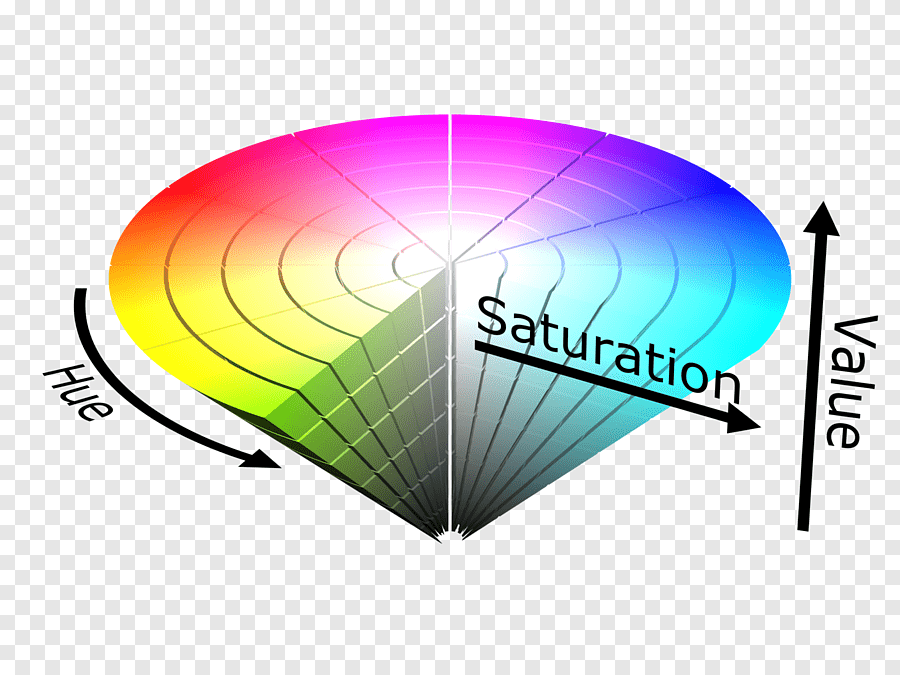
\includegraphics[width=0.5\textwidth]{imagens/HSV.png} 
    \caption{HSV Color Pattern} 
\end{figure}

\newpage
\textbf{Grayscale} - 
Grayscale is a single-channel image format that removes all hue and saturation, leaving only its brightness value, by reducing the three channels down to only one~\cite{deep2025intellimotion}, it greatly decreases the processing load, and its increased simplicity enables the creation of color masks that can filter out backgrounds and simplify complex objects for easier analysis, this is a fundamental pre-processing step for Algorithm and Deep Learning training.

\begin{figure}[h]
    \centering 
    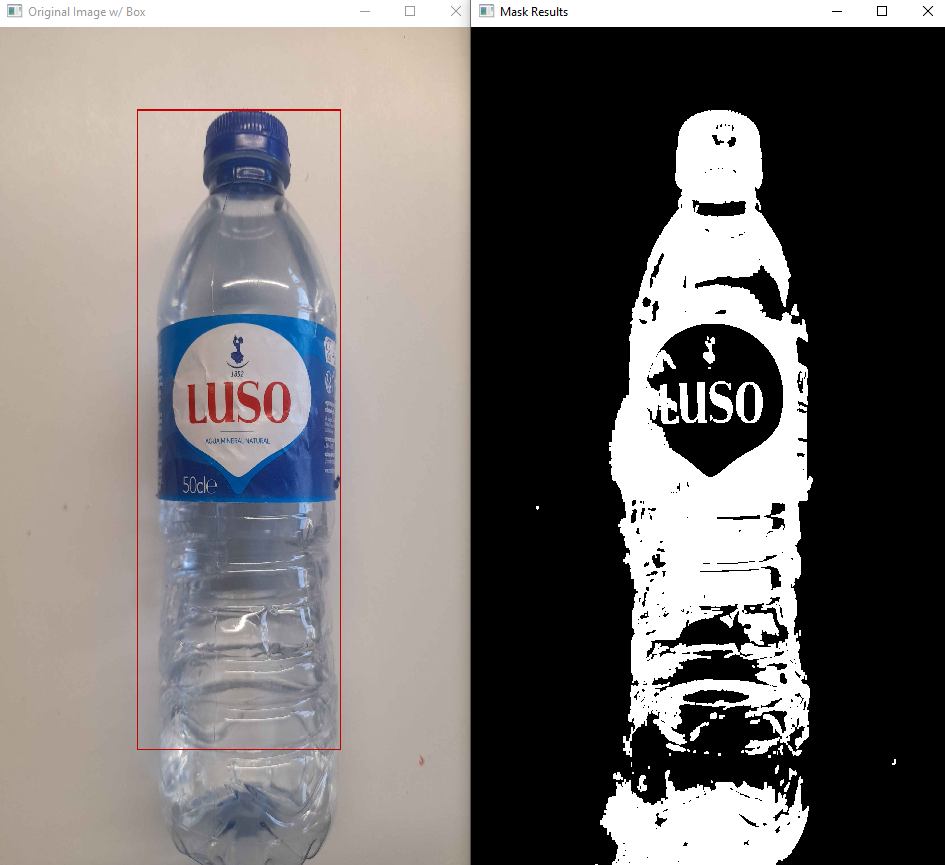
\includegraphics[width=0.5\textwidth]{imagens/Color Mask Example.png} 
    \caption{Color Mask Example using Grayscale} 
\end{figure}

\subsubsection{Inference}
Inference is the process where an AI Algorithm makes predictions based on the data provided, in this project, the data consists of the live feed being captured by the camera, which is continuously being fed into the model for analysis, because of the nature of this software, the inference must be done with relatively high speed and precision to ensure low latency and smooth operation.

\subsubsection{Landmarks}
The last step of the analysis is show its results, once Inference is done correctly, the model will return 21 sets of coordinates (x,y,z), these are landmarks spread throughout the hand, from the wrist to the finger tips, the software then reconstructs the hand gesture by connecting these coordinates together, creating a uniform pattern that will allow us to use a model and recognize what motion or gesture the hand is making.

\subsection{State-of-the-Art}

\subsubsection{VSCode \& Python}
VSCode is a lightweight but versatile Integrated Development Environment (IDE) with support for hundreds of languages. Python is one of the most widely used programming languages, known for its versatility, fast prototyping, and beginner friendly, it was chosen for having better integration with OpenCV and MediaPipe, and being able to perform complex mathematical operations while maintaining a fast performance.

\subsubsection{OpenCV}
OpenCV is an Open Source Computer Vision Library that acts as the eyes for this project, as well as the bridge between the camera feed and the software, it's responsible for the frame acquisition, its pre-processing, the drawing of the model inference results, as well as displaying the softwares' logic directly onto the video feed, the library has more than 2500 algorithms and it's a versatile tool that works efficiently with other AI Models for a wide range of computer vision projects, from object detection to face recognition, this tool was chosen for its ease-of-use, optimized real-time performance and image processing~\cite{opencv_about}.
	
\subsubsection{MediaPipe Model}
MediaPipe is an open source framework developed by Google, it specializes in real time, machine learning solutions for live video, audio and streaming~\cite{mediapipe_main}, for this project it uses an Inference engine for hand tracking, it uses a palm detector and a landmark model to draw 21 points throughout the image of a hand with very low latency~\cite{mediapipe_hands}, which enables it to work in tandem with the camera and OpenCV to continuously analyze the images and display the results at a very high speed~\cite{deep2025intellimotion}.

% 3. Outlook of the technology
\section{Outlook of the technology}
% (provide a snapshot of the main characteristics/functionality of the technology described in this lab script)

\subsection{Setup/Installation (SW/HW)}
% (describe the way to start using the technology, namely the setpup/installation SW/HW requirements, operating systems, development platforms,…)

\subsubsection{Windows Setup}
To start the lab script, students must ensure their Windows workstations meet the following requirements:

Hardware Requirements:
\begin{itemize}
    \item A personal computer (desktop or laptop).
    \item A video camera (built-in or USB peripheral).
    \item An active connection to a Local Area Network (LAN), either via Wi-Fi or an Ethernet cable.
\end{itemize}

Software and Development Platform Requirements:
\begin{itemize}
    \item Operating System: Microsoft Windows (Windows 10 or 11 is recommended).
    \item Platform: Python 3.8 (or higher) installed. During the installation process, it is strictly necessary to check the "Add Python to PATH" option to allow the execution of global commands, as shown in Figure \ref{fig:python_path}.
    
    \begin{figure}[h]
        \centering
        % Aqui o LaTeX vai buscar a tua primeira imagem!
        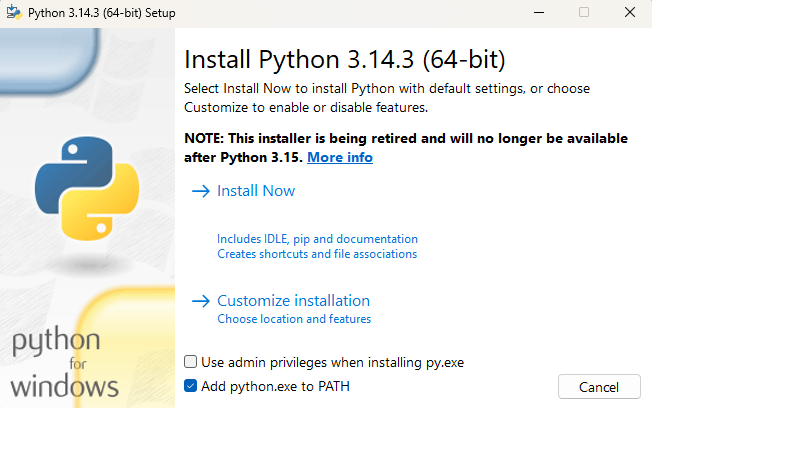
\includegraphics[width=0.6\textwidth]{imagens/python.png}
        \caption{Adding Python to PATH during installation.}
        \label{fig:python_path}
    \end{figure}

    \item Environment: An Integrated Development Environment (IDE) such as Visual Studio Code (VS Code) is recommended.
    \item Dependencies: The computer vision libraries must be installed via the Windows Command Prompt (\texttt{cmd}) or PowerShell. The student must execute the following command using the \texttt{pip} package manager, as demonstrated in Figure \ref{fig:cmd_pip}:
    
    \begin{figure}[h]
        \centering
        % Aqui o LaTeX vai buscar a tua segunda imagem!
        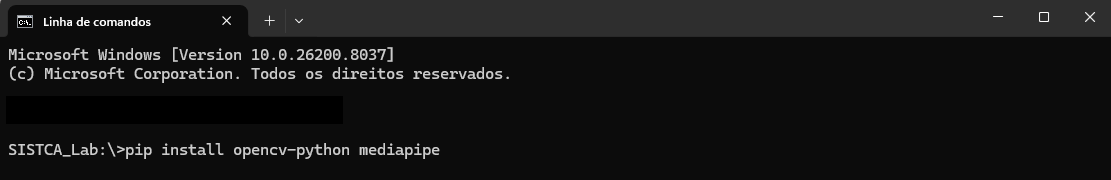
\includegraphics[width=0.8\textwidth]{imagens/cmd.png}
        \caption{Installing required libraries via Command Prompt.}
        \label{fig:cmd_pip}
    \end{figure}
\end{itemize}

\subsubsection{Linux Setup}
If you are using Linux we'll assume you have a basic understanding of the command line and already have Visual Studio Code installed, so you can follow these steps to set up your environment:
\begin{enumerate}
    \item Choose or create the directory where you want to create your project.
    \item Open a terminal and make sure your system is up to date by running:
    \begin{lstlisting}[language=bash]
# Linux Update Commands
@sudo@ apt update
@sudo@ apt upgrade
    \end{lstlisting}
    \item Install Python and pip if you haven't already:
    \begin{lstlisting}[language=bash]
# Linux Python Installation Commands
@sudo@ apt install python3 python3-pip python3-venv
    \end{lstlisting}
    \item Inside your project directory, open a terminal and create a virtual environment for your project (optional but recommended):
    \begin{lstlisting}[language=bash, ]
# Linux Virtual Environment Commands
@python3@ -m venv myvenv
@source@ myvenv/bin/activate
    \end{lstlisting}
    \item \sloppy Inside Visual Studio Code (\textit{in your project directory}), open the Command Palette (Ctrl+Shift+P) and select ``Python: Select Interpreter''. Choose the interpreter from your virtual environment (it should be something like \textbf{`myvenv/bin/python`}).
    \item Upgrage pip and install the following packages:
    \begin{lstlisting}[language=bash]
# Linux Package Installation Commands
@pip@ install --upgrade pip
@pip@ install opencv-python mediapipe scikit-learn pandas
    \end{lstlisting}
\end{enumerate}


\subsection{First Steps}

The development of the Hand-Tracking Software begins with the use of the \textbf{OpenCV} library alongside the front-facing camera to obtain a video feed in real-time, aiming to continuously capture hand movements and gestures.

The function \verb|cap = cv2.VideoCapture(n)| is responsible for the camera initialization. The index $n=0$ refers to built-in webcams commonly found in laptops, whereas higher indexes ($n=1,2,...$) allow access to secondary cameras connected via USB. It's crucial for both the camera and processor to capture the images at a high framerate to ensure smooth hand tracking and increased precision for analysis.

Before sending the image to the algorithm, pre-processing is required. OpenCV captures frames in the \textbf{BGR} format (Blue, Green, Red). The function \verb|cv2.cvtColor(frame, cv2.COLOR_BGR2RGB)| will convert it to the \textbf{RGB} format (Red, Green, Blue), which is the standard format used by most Deep Learning Models to ensure correct Inference (AI Processing). In addition, mirroring the frame with the function \verb|cv2.flip(frame, 1)| provides a more intuitive feed for the user.

\begin{lstlisting}[title={Basic Camera Feed using OpenCV}, language=Python, captionpos=b]
import cv2

cap = cv2.VideoCapture(0)
cv2.namedWindow('Hand Tracker', cv2.WINDOW_NORMAL)

while True:
    ret, frame = cap.read()
    if not ret:
        print("Error: Failed to grab frame.")
        break
 
    frame = cv2.flip(frame, 1)
    rgb_frame = cv2.cvtColor(frame, cv2.COLOR_BGR2RGB)

    cv2.imshow('Hand Tracker', frame)
    if cv2.waitKey(1) & 0xFF == ord('q'):
        break

cap.release()
cv2.destroyAllWindows()
\end{lstlisting}

The next step is to pass the frames through the MediaPipe model, which analyses the image and returns 21 Hand Landmarks placed throughout the hand, storing their respective coordinates. The analysis is triggered by calling the function \verb|results = hands.process(rgb_frame)|. Following the Inference, if a hand is detected, the coordinates are connected by lines and drawn onto the original frame, which is then displayed in the window feed.

\begin{lstlisting}[title={Mediapipe Frame Analysis}, language=Python, captionpos=b]
import cv2
import mediapipe as mp

# MediaPipe Model Config
mp_hands = mp.solutions.hands
mp_drawing = mp.solutions.drawing_utils
hands = mp_hands.Hands(min_detection_confidence=0.9, min_tracking_confidence=0.9)

# MediaPipe Coordinates to Finger Tip ID (Index, Middle, Ring, Pinky)
finger_tips = [8, 12, 16, 20]
thumb_tip = 4

# OpenCV Camera Feed
cap = cv2.VideoCapture(0)

while cap.isOpened():
    ret, frame = cap.read()
    if not ret: break
    
    frame = cv2.flip(frame, 1)
    rgb_frame = cv2.cvtColor(frame, cv2.COLOR_BGR2RGB)
    results = hands.process(rgb_frame)

    if results.multi_hand_landmarks:
        # We use 'enumerate' to know which hand we're looking at
        for hand_idx, hand_landmarks in enumerate(results.multi_hand_landmarks):
            
            # Draw Lines and Coordinates in Hand
            mp_drawing.draw_landmarks(frame, hand_landmarks, mp_hands.HAND_CONNECTIONS)

            # Find which hand (left or right) is being detected
            hand_label = results.multi_handedness[hand_idx].classification[0].label
            raised_fingers = 0

            # 1. Thumb Logic (X-Axis)
            if hand_label == "Right":
                if hand_landmarks.landmark[thumb_tip].x < hand_landmarks.landmark[thumb_tip - 1].x:
                    raised_fingers += 1
            else: # "Left"
                if hand_landmarks.landmark[thumb_tip].x > hand_landmarks.landmark[thumb_tip - 1].x:
                    raised_fingers += 1

            # 2. Other 4 Fingers Logic (Y-Axis)
            for tip in finger_tips:
                # On the Window, the Y-Axis increases downward
                if hand_landmarks.landmark[tip].y < hand_landmarks.landmark[tip - 2].y:
                    raised_fingers += 1

            # Write Text in Window
            cv2.putText(frame, f'{hand_label} hand: {raised_fingers} fingers', 
                       (10, 50 + (hand_idx * 50)),
                       cv2.FONT_HERSHEY_SIMPLEX, 1, (0, 255, 0), 2, cv2.LINE_AA)

    cv2.imshow('Hand Tracker', frame)
    if cv2.waitKey(1) & 0xFF == ord('q'): break

cap.release()
cv2.destroyAllWindows()
\end{lstlisting}

This continuous cycle of frame acquisition and immediate algorithmic analysis makes up the fundamental core of this project. The following chapter will elaborate on how the 21 hand landmarks can be used to detect patterns and movements. By leveraging this data, we can send commands to the computer, enabling control over the system through hand gestures alone.

% 4. Tutorial/Functionality
\section{Tutorial/Functionality}
\label{sec:tutorial_advanced}

In this chapter, we will dissect the codebase developed for real-time hand detection and finger counting. Beyond simply presenting the code, this section elucidates the underlying algorithmic thought process and details the fundamental commands provided by the \textbf{OpenCV} and \textbf{MediaPipe} libraries.

\subsection{Algorithmic Rationale}
Before delving into the syntactic implementation, it is crucial to understand the logical pipeline of the system:
\begin{enumerate}
    \item \textbf{Data Acquisition:} Capture a continuous stream of visual data from a hardware peripheral (webcam).
    \item \textbf{Normalization:} Mirror the image for intuitive user interaction and convert the color space to meet the machine learning model's prerequisites.
    \item \textbf{Inference:} Pass the normalized image through the MediaPipe neural network to extract a topological graph of the hand (landmarks).
    \item \textbf{Kinematic Evaluation:} Utilize the spatial coordinates of these landmarks to deduce the state of each digit (extended or folded) based on anatomical constraints.
    \item \textbf{Feedback:} Overlay the computed state onto the original image stream to provide real-time visual feedback.
\end{enumerate}

\subsection{Environment Setup and Core Libraries}
\label{subsec:setup}

We initiate the script by importing the requisite libraries and defining the core MediaPipe objects.

\begin{lstlisting}
import os
os.environ["QT_QPA_PLATFORM"] = "xcb" 

import cv2
import mediapipe as mp

mp_hands = mp.solutions.hands
mp_drawing = mp.solutions.drawing_utils
hands = mp_hands.Hands(min_detection_confidence=0.5, min_tracking_confidence=0.5)
\end{lstlisting}

\textbf{Basic Commands Explained:}
\begin{itemize}
    \item \texttt{import cv2}: Imports the OpenCV library, the industry standard for real-time computer vision and image processing tasks.
    \item \texttt{mp.solutions.hands}: Accesses the specific hand tracking module within the broader MediaPipe framework.
    \item \texttt{mp\_hands.Hands(...)}: Instantiates the machine learning model. The parameters \texttt{min\_detection\_confidence} and \texttt{min\_tracking\_confidence} act as statistical thresholds. Setting them to $0.5$ dictates that the model must be at least 50\% certain that a hand is present to begin or continue tracking it, balancing processing speed with accuracy.
\end{itemize}

\subsection{Video Capture and Landmark Mapping}
\label{subsec:capture}

The subsequent phase involves initializing the hardware interface and establishing the indices for the finger landmarks.

\begin{lstlisting}
cap = cv2.VideoCapture(1)
cv2.namedWindow('Hand Tracker', cv2.WINDOW_NORMAL)

# IDs for the fingertip landmarks in MediaPipe (Index, Middle, Ring, Pinky)
pontas_dos_dedos = [8, 12, 16, 20]
ponta_do_polegar = 4
\end{lstlisting}

\textbf{Basic Commands Explained:}
\begin{itemize}
    \item \texttt{cv2.VideoCapture(1)}: Creates a video capture object. The argument \texttt{1} targets the secondary camera interface, while \texttt{0} typically targets the primary built-in webcam.
    \item \texttt{cv2.namedWindow(...)}: Initializes a graphical user interface (GUI) window. The \texttt{WINDOW\_NORMAL} flag allows the user to resize the output window dynamically.
\end{itemize}

\subsection{Image Pre-processing: The "Why" and "How"}
\label{subsec:preprocessing}

Within the continuous execution loop (\texttt{while True}), raw frames are acquired and mathematically transformed.

\begin{lstlisting}
while True:
    ret, frame = cap.read()
    if not ret:
        break

    frame = cv2.flip(frame, 1)
    rgb_frame = cv2.cvtColor(frame, cv2.COLOR_BGR2RGB)
    results = hands.process(rgb_frame)
\end{lstlisting}

\textbf{Thought Process \& Basic Commands:}
\begin{itemize}
    \item \texttt{cap.read()}: Extracts the subsequent frame from the video stream. It returns a boolean (\texttt{ret}) indicating success, and the matrix of pixels (\texttt{frame}).
    \item \texttt{cv2.flip(frame, 1)}: Applies a horizontal mirror reflection across the vertical axis (indicated by the \texttt{1}). Without this operation, moving your hand to the left would result in the on-screen hand moving to the right, which causes severe cognitive dissonance for the user.
    \item \texttt{cv2.cvtColor(...)}: OpenCV natively captures color arrays in Blue-Green-Red (BGR) format. However, the MediaPipe neural network was trained on Red-Green-Blue (RGB) datasets. This function strictly translates the color channels to ensure the model processes the image accurately.
    \item \texttt{hands.process(rgb\_frame)}: Executes the core inference step, passing the RGB matrix into the neural network and returning a \texttt{results} object containing the spatial coordinates of any detected hands.
\end{itemize}

\subsection{Kinematic Logic: The Coordinate System}
\label{subsec:logic}

When hands are detected, the algorithm iterates through them and evaluates the spatial configuration of the digits.

\begin{lstlisting}
    if results.multi_hand_landmarks:
        for hand_idx, hand_landmarks in enumerate(results.multi_hand_landmarks):
            mp_drawing.draw_landmarks(frame, hand_landmarks, mp_hands.HAND_CONNECTIONS)

            hand_label = results.multi_handedness[hand_idx].classification[0].label
            dedos_levantados = 0

            # 1. Thumb Logic (X-Axis)
            if hand_label == "Right":
                if hand_landmarks.landmark[ponta_do_polegar].x < hand_landmarks.landmark[ponta_do_polegar - 1].x:
                    dedos_levantados += 1
            else: # "Left"
                if hand_landmarks.landmark[ponta_do_polegar].x > hand_landmarks.landmark[ponta_do_polegar - 1].x:
                    dedos_levantados += 1

            # 2. Logic for the remaining 4 fingers (Y-Axis)
            for ponta in pontas_dos_dedos:
                if hand_landmarks.landmark[ponta].y < hand_landmarks.landmark[ponta - 2].y:
                    dedos_levantados += 1
\end{lstlisting}

\textbf{Thought Process for Finger Counting:}
The algorithm's core logic is predicated on the digital image coordinate system, where the origin $(0,0)$ is located at the top-left corner of the image. Consequently, moving downwards increases the Y-value, and moving rightwards increases the X-value.

\begin{itemize}
    \item \textbf{The Four Fingers (Index to Pinky):} To determine if a finger is "up", we compare the Y-coordinate of the fingertip (\texttt{landmark[ponta]}) to the Y-coordinate of the knuckle two joints below it (\texttt{landmark[ponta - 2]}). Due to the inverted Y-axis, a numerically smaller Y-value indicates a higher physical position. Thus, if $Y_{tip} < Y_{knuckle}$, the finger is extended.
    \item \textbf{The Thumb Anomaly:} The thumb operates on a different biomechanical plane, rotating horizontally rather than folding vertically. Therefore, we evaluate the X-axis. A right thumb pointing leftwards (towards the center of the body) has a smaller X-value than its base joint. This logic must be strictly inverted for the left hand, necessitating the \texttt{hand\_label} conditional check.
\end{itemize}

\subsection{Visual Output and Resource Deallocation}
\label{subsec:output}

Finally, the extracted data is overlaid onto the original BGR frame for the user's viewing.

\begin{lstlisting}
            cv2.putText(frame, f'{hand_label} hand: {dedos_levantados} fingers', (10, 50 + (hand_idx * 50)),
                        cv2.FONT_HERSHEY_SIMPLEX, 1, (0, 255, 0), 2, cv2.LINE_AA)

    cv2.imshow('Hand Tracker', frame)

    if cv2.waitKey(1) & 0xFF == ord('q'):
        break

cap.release()
cv2.destroyAllWindows()
\end{lstlisting}

\textbf{Basic Commands Explained:}
\begin{itemize}
    \item \texttt{cv2.putText(...)}: Renders text directly onto the pixel matrix. The algorithmic offset \texttt{50 + (hand\_idx * 50)} ensures that if multiple hands are detected, their respective text labels stack vertically without visual occlusion.
    \item \texttt{cv2.imshow(...)}: Commands the operating system to refresh the GUI window with the newly processed frame.
    \item \texttt{cv2.waitKey(1)}: Halts execution for 1 millisecond to listen for keyboard interrupts. If the user presses the 'q' key, the \texttt{while} loop breaks.
    \item \texttt{cap.release() \& cv2.destroyAllWindows()}: These cleanup functions are crucial; they sever the connection to the hardware camera to prevent system locks and safely close all active graphical windows.
\end{itemize}

\subsection{Advanced Integration: Custom AI Model and Mouse Control (HCI)}

While in Section 4.5 successfully count fingers, they are highly dependent on 2D perspective and camera angles. To make the system truly robust, we can replace these hardcoded rules with a custom Machine Learning (ML) model and utilize the predictions for Human-Computer Interaction (HCI), specifically controlling the operating system's mouse pointer.

\subsubsection{Feature Engineering (Wrist Relativity)}
To train a robust model, the input data must be position-invariant. If raw screen coordinates are fed into the model, the algorithm will overfit to the hand's pixel location on the screen rather than learning its structural shape. 

We set the wrist (Landmark 0) as the origin point $(0,0,0)$. All other 20 landmarks are calculated relative to the wrist using the following transformations:

\begin{align}
    x_{rel} &= x_i - x_{wrist} \\
    y_{rel} &= y_i - y_{wrist} \\
    z_{rel} &= z_i - z_{wrist}
\end{align}

\begin{lstlisting}[language=Python, caption=Extracting 3D Position-Invariant Features]
landmark_data = []
wrist = hand_landmarks.landmark[0]

for landmark in hand_landmarks.landmark:
    rel_x = landmark.x - wrist.x
    rel_y = landmark.y - wrist.y
    rel_z = landmark.z - wrist.z
    landmark_data.extend([rel_x, rel_y, rel_z])
\end{lstlisting}

\subsubsection{Training the Classifier}
By capturing a dataset containing roughly 100-200 variations of each gesture (0 to 5 fingers) using these engineered relative coordinates, the data becomes tabular. This allows us to utilize the \texttt{scikit-learn} library to train a Random Forest Classifier.

\begin{lstlisting}[language=Python, caption=Training a Random Forest Model]
import pandas as pd
from sklearn.model_selection import train_test_split
from sklearn.ensemble import RandomForestClassifier
import pickle

# Load dataset and split into 80% Training and 20% Testing
df = pd.read_csv('hand_data.csv')
X = df.drop('label', axis=1) 
y = df['label']              
X_train, X_test, y_train, y_test = train_test_split(X, y, test_size=0.2, random_state=42)

# Train the model
model = RandomForestClassifier(n_estimators=100, random_state=42)
model.fit(X_train, y_train)

# Save the trained model
with open('hand_model_3d.pkl', 'wb') as f:
    pickle.dump(model, f)
\end{lstlisting}

\subsubsection{Real-Time Mouse Control (HCI)}
With a trained model (\texttt{.pkl} file) capable of recognizing gestures, we can import the \texttt{pyautogui} library to bridge the gap between Python and the operating system. 

The tip of the index finger (Landmark 8) dictates the cursor's spatial $X$ and $Y$ coordinates, mapped to the monitor's resolution. When the ML model classifies the hand structure as a closed fist ("0"), the script triggers a left-click event.

\begin{lstlisting}[language=Python, caption=HCI Mouse Control Integration]
import pyautogui
import time

# Mouse mapping logic using the Index Finger
index_finger_tip = hand_landmarks.landmark[8]
mouse_x = int(index_finger_tip.x * screen_w)
mouse_y = int(index_finger_tip.y * screen_h)
pyautogui.moveTo(mouse_x, mouse_y, _pause=False)

# Clicking logic based on ML prediction
if prediction == '0':
    if (current_time - last_click_time) > 1.0: # 1-second cooldown
        pyautogui.click()
        last_click_time = current_time
\end{lstlisting}

% 5. Exercise(s)
\section{Exercise(s)}
\subsection{Problem A - Alt Tab Command}
In this setting of using our hands to control our computer, the ability to "alt-tab" anytime is a very useful feature that allows the user to navigate the entire workspace in an instant. For this exercise, we want to map this command to a finger or a gesture, so that we can still use the index finger to control the mouse cursor around the screen.

\subsubsection{Resolution A}
Using the Ring Finger (Landmark 16), we can create a simple geometric rule to trigger the Alt-Tab keyboard macro using PyAutoGUI.

\begin{lstlisting}[caption={Exercise A - Alt Tab Implementation}, language=Python, captionpos=b]
rf_point = hand_landmarks.landmark[16] # Ring Finger Tip
rf_base = hand_landmarks.landmark[14]  # Ring Finger PIP Joint (Base)

# If Point is Higher than Base, Ring Finger is raised: Activate Command
if rf_point.y < rf_base.y:             
    # Flag controls Alt key press status, so it doesnt conflict with normal computer use
    if not f_alttab:              
        pyautogui.keyDown('alt')       # Presses Alt key, keeps it pressed
        pyautogui.press('tab')         # Presses Tab key once to enter menu
        f_alttab = True                # Activates Flag
else:
    if f_alttab:
        pyautogui.keyUp('alt')         # Releases Alt key if it was pressed
        f_alttab = False               # Deactivates Flag
\end{lstlisting}

\subsection{Problem B - Screenshot Automation}
Enhance the existing real-time hand-tracking and mouse-control software to trigger a screenshot when a specific gesture is detected. The system needs to recognize when the user fully extends their pinky finger and then execute the \texttt{Windows + Shift + S} keyboard shortcut. Importantly, the program must continue running right after pressing the shortcut. This allows the user to use the existing hand gestures to move the mouse and select the area for the screenshot.

\subsubsection{Resolution B}
To add this feature, we use the \texttt{pyautogui} library to simulate keyboard presses. The logic depends on checking the position of the pinky finger using the MediaPipe hand tracking model. 

According to the model, the tip of the pinky finger is point (landmark) 20. We can figure out if the finger is raised by comparing the Y-coordinate of the tip (landmark 20) with a lower joint, like landmark 18. In images, the Y-axis goes from top to bottom, meaning a smaller Y-value is physically higher on the screen. So, if the tip's Y-value is smaller than the joint's Y-value, the finger is raised.

A major challenge is preventing the shortcut from triggering multiple times a second without pausing the video feed. If we use a simple \texttt{time.sleep()} function, the whole program freezes. This would stop the camera and the mouse control, making it impossible to crop the screenshot. Instead, we use a non-blocking timer with \texttt{time.time()}. This method checks the current time and ensures the shortcut is only pressed once every few seconds. Because the main loop never stops, the user can immediately close their hand (which our Custom AI model predicts as state \texttt{0}) to click and drag the mouse to capture the screen.

The code modification required to implement this logic within the existing software is shown below:
\begin{lstlisting}[caption={Exercise B - Screenshot Automation Implementation}, language=Python, captionpos=b]
import pyautogui
import time

# --- Setup Configuration (Place before the main while loop) ---
pyautogui.PAUSE = 0 
last_action_time = 0
COOLDOWN_SECONDS = 2.0

# ... [Inside the 'for hand_landmarks in results.multi_hand_landmarks:' loop] ...

# 1. Check if the pinky finger is raised
pinky_tip = hand_landmarks.landmark[20].y
pinky_pip = hand_landmarks.landmark[18].y
is_pinky_raised = pinky_tip < pinky_pip

current_time = time.time()

# 2. Trigger the shortcut with a non-blocking timer
if is_pinky_raised and (current_time - last_action_time > COOLDOWN_SECONDS):
    pyautogui.hotkey('win', 'shift', 's')
    last_action_time = current_time # Reset the cooldown timer

# ... [The rest of the existing gesture control logic remains unchanged] ...
\end{lstlisting}

This approach allows the software to take a screenshot and immediately transition back to gesture control, fulfilling the exercise requirements while keeping the application smooth and responsive[cite: 430, 431].

% 6. Challenge
\section{Challenge: The "Virtual Zoom"}

To conclude this lab script, the final challenge consists of expanding the system's capabilities, focusing on accessibility and document navigation.

\vspace{0.4cm}
\textbf{Problem Statement:} 
When analyzing complex electrical schematics or reading technical documentation, it is often necessary to zoom in or out without taking your hands off the task being performed. The objective is to modify the \texttt{run\_ai.py} script to function as a gesture-controlled magnification tool.

\vspace{0.6cm}
\textbf{Requirements and Objectives:}
\begin{itemize}
    \item \textbf{Movement 1 and Command 1 (Zoom In):} Detect when the user's hand is fully open (5 fingers raised). This movement must trigger the \texttt{Ctrl +} shortcut via the \texttt{pyautogui.hotkey('ctrl', '+')} command.
    \item \textbf{Movement 2 and Command 2 (Zoom Out):} Detect when the user's hand is fully closed (0 fingers raised). This movement must trigger the \texttt{Ctrl -} shortcut via the \texttt{pyautogui.hotkey('ctrl', '-')} command.
    \item \textbf{Cooldown Implementation:} As learned in Exercise B, you must implement a non-blocking timer using \texttt{time.time()} to prevent the command from being triggered multiple times per second. A cooldown interval of at least 1.2 seconds is recommended.
\end{itemize}

\vspace{0.4cm}
\textbf{Implementation Hint:} You can solve this challenge by checking your Machine Learning model's output variable (\texttt{prediction}). Confirm if the string value is exactly \texttt{'5'} or \texttt{'0'} before executing the respective shortcut command and resetting the non-blocking timer.
\newpage
% 7. References
\bibliographystyle{ieeetr}
\bibliography{references}

\newpage
% Annexes
\section*{Annexes}
\addcontentsline{toc}{section}{Annexes}
% (here you should include any technical documentation that you consider relevant for supporting the lab script but does not “fit into”, as you feel it would jeopardize the reading flow of the core text)

\end{document}